\documentclass[onecolumn,10pt]{IEEEtran}

\usepackage{amsmath,amsfonts,amssymb}
\usepackage{graphicx}
%\usepackage{marginnote} % for editorial use
\usepackage{sidenotes} % for editorial use
\usepackage[dvipsnames,svgnames]{xcolor}
\usepackage{svg,svg-extract}
\usepackage{booktabs}

\usepackage{siunitx}
\DeclareSIUnit\foot{ft}
\DeclareSIUnit\pound{lb}
\DeclareSIUnit\ounce{oz}
\DeclareSIUnit\inch{in}
\DeclareSIUnit\rpm{rpm}
\DeclareSIUnit\fahrenheit{F}
\DeclareSIUnit\bit{bit}
\DeclareSIUnit\byte{B}

\newcommand{\myroot}{../}
\newcommand{\Later}{\textbf{Later.}}
\newcommand{\Calypteanna}{\emph{Calypte anna}}
\newcommand{\Canna}{\emph{C.~anna}}
\newcommand{\MATLAB}{Matlab}
\newcommand{\Matlab}{Matlab}

\usepackage{hyperref}
\hypersetup{
  colorlinks=true,
  linkcolor=violet,
  urlcolor=blue,
  citecolor=blue}

\usepackage[plain]{fancyref}
\renewcommand{\freffigname}{Fig.}
\renewcommand{\Freffigname}{Fig.} 
\renewcommand{\freftabname}{Table}
\renewcommand{\Freftabname}{Table}
\frefformat{plain}{\fancyrefeqlabelprefix}{(#1)} 
\Frefformat{plain}{\fancyrefeqlabelprefix}{(#1)} 

\usepackage{listings}
\lstset{
	basicstyle=\ttfamily,
	columns=fullflexible,
	showstringspaces=false
}
\lstdefinestyle{mbedC}{
	language=C,
	basicstyle=\ttfamily,
	keywordstyle=\color{blue}\ttfamily,
	stringstyle=\color{magenta}\ttfamily,
	commentstyle=\color{green}\ttfamily,
	directivestyle=\color{red}\ttfamily,
 	morecomment=[l][\color{red}]{\#},
	columns=fullflexible,
	showstringspaces=false,
%	frame=single
}
\lstdefinestyle{usnaMatlab}{
	basicstyle=\ttfamily,
	keywordstyle=\color{blue}\ttfamily,
	stringstyle=\color{magenta}\ttfamily,
	commentstyle=\color{green}\ttfamily,
 	morecomment=[l][\color{red}]{\#},
	columns=fullflexible,
	showstringspaces=false,
	language=Matlab
%	%backgroundcolor=\color{lightgray},
%	frame=single
}


\title{Autonomous drone racing}
\author{A.~Credle and D.~Evangelista\thanks{Authors are with the United States Naval Academy, Department of Weapons, Robotics, and Control Engineering}}
\date{\today}


% For EW495 title page
\usepackage{titlepage4956}
\coursenumber{EW495}
\student{MIDN 1/C Credle}
\advisor{Assistant Professor D. Evangelista}
\coverpicture{\includegraphics[width=4.48in]{titlepage.png}}


\begin{document}
\maketitlepage
\maketitle

\begin{abstract}
Autonomous racing drones are not only beneficial to the drone racing sport, but also in autonomous vehicles and in military drones flying through windows, chimneys, etc. Research in this field is often based around either race gate recognition or flight controls, but this project will incorporate both. We will create a process for a drone to modify its given flight path based on the visual recognition of the gate in order to fly through the gate. The processor will identify the gate, locate it in relation to the drone’s current path, and modify the path to fly through the gate. This project will demonstrate this process by using simulations and physical experiments. Simulations will consist of individual tests of recognition, location, and path modification processes, and then tests for all three together. Physical experiments will test all three process together in a real environment. Success will be measured by the difference in distance between the path and the center of the gate, as well as the difference in trajectory at the same point. The total cost of the project is \$29,666 with \$1586 of that being new equipment. This project is scheduled to have the coding and simulation done within the first semester and physical experiments done by the end of the second. The biggest risk involved is with the drones crashing, so the physical experiments have more time than simulations to ensure safety. If successful, this will be the first step in creating an autonomous racing drone at USNA.
\end{abstract}

\begin{IEEEkeywords}
capstone, robotics, controls
\end{IEEEkeywords}

\section{Introduction}
\subsection{Background and motivation}
    The concept of drone racing is straightforward: a group of people fly unmanned aerial vehicles (UAV) through gates, the first one to the finish line wins. The UAVs, or drones, come in a variety of sizes, ranging from an inch in diameter to over a foot, and are flown through communication with a remote controller. Races can take place in a variety of conditions including time of day and location. Gates can be configured in an unlimited number of patterns and often come in circular or rectangular form, though they are not limited to these shapes. Limitations are often placed on the power and size of drones that are raced, as owners are often expected to bring their own equipment \cite{redbull2018drone}. While the concept of racing is not new, drone racing is one of the fastest growing sports in the world \cite{condliffe2016is}. Its fame is quickly growing, and sports broadcasting companies like ESPN are signing contracts to broadcast competitions \cite{marshall2017espn}. There are no limitations on age, gender, ethnicity, or physical prowess, making drone racing available to everyone.
\begin{figure}[hb]
\begin{center}
\includegraphics[width=4.14in]{fig1.png}
\end{center}
\caption{Two drones racing}
\label{fig:1}
\end{figure}

The concept of autonomous drone racing is even newer, though its potential goes beyond that of its sport. In concept, a human drone racer goes through a series of cues and maneuvers to race the drone. If these cues and maneuvers are broken down into systematic steps, it is possible to automate the process and have the drone fly itself through the course. In modern autonomous vehicles, the specific location of the vehicle is often known, through GPS, a tracking system, etc. While this method of localization works for vehicles with static environments, it does not take into account the location of its surrounds, or the vehicles location in relation to specific objects. 

By mixing both an assumed path and gates for the drone to fly through, the exact location of the drone is not required; its relative location to the gates is all that is needed to fly a successful race. This concept will be critical for future autonomous systems, such as self-driving cars, that are required to navigate based on an assumed path mixed with the vehicles relative to the environmental objects or barriers (\fref{fig:1}) \cite{iot2018how}. For cars, the environmental objects would include lane lines, other vehicles, curbs, objects in the road, etc \cite{rayej2014how}. By integrating objects of the environment into the core of the navigation process, autonomous vehicles will be able to keep both passengers, pedestrians, and wildlife safe. Autonomous vehicles of the future must be able to navigate based on both an assumed path and a relative location in order to efficiently and safely navigate dynamic environments.  
\begin{figure}[hb]
\begin{center}
\includegraphics[width=3.90in]{fig2.png}
\end{center}
\caption{An autonomous car sensing its environment}
\label{fig:2}
\end{figure}

As the first autonomous drone-racing project at USNA, this will open the door to future drone research for midshipmen. EW281 and EW282 provide opportunities for midshipmen to experiment with drones on a hardware and flight-testing level, but this project will allow for future drone development on the software and autonomy level. Additionally, this research is only the first step in creating a fully autonomous racing drone that rivals a human’s performance. Future steps include path optimization, recognition with visual uncertainties, racer collision avoidance, etc. This research will be one small step in the larger picture of fully autonomous drone racing.

\subsection{Problem statement}
Given a three-dimensional flight path, drone accelerometer readings, and the image of a drone-racing gate in a three dimensional environment, this research intends to begin the process of developing autonomous drone flight through a drone-racing course. Given a three-dimensional path that does not fly through the gate, we will find and test the feasibility of a guidance system that creates a similar path that does. This system will be tested by placing a small quadrotor in multiple scenarios in relation to a race gate(s), with varying pre-determined paths, and directing the guidance system to fly the drone through the race gate(s). Success of this system is based on the ability to autonomously correct the path and fly the drone through the center of the gate without contact. This will be measured by the difference in distance between the path at its intersection with the gate, and the center of the gate. The competing objective will be to maintain the same trajectory at the intersection with the gate as if the path had not been modified. The final output of this project will a guidance system that could be implemented on any racing drone with a camera and IMU and fly through race gates autonomously.
\begin{figure}[t]
\begin{center}
\includegraphics[width=4in]{fig3.png}
\end{center}
\caption{Depiction of flight path correction (original path in green, new path in blue, trajectory at gate intersection as red arrow, gate intersection point as red dot)}
\label{fig:3}
\end{figure}

\subsection{Literature review}
This paper is the one of the first developments of a drone autonomous flight program, so the background research encompasses papers that focus on multiple aspects of autonomous flight. The main categories that these papers include navigation, flight controls, and visual recognition. This research focuses on the visual recognition of the gate and navigation, but these flight controls is necessary for the background research because it affect the performance of navigation and is necessary for basic demonstration.

In order to understand the movement patterns of the drone, \cite{svacha2017improving} provides a set of equations that could be used to accurately model the induced drag and thrust forces. These equations were derived from proofs using properties of physics, and then the coefficients were identified through flight experimentation. This provides suitable estimations for the forces acting on the drone, which allows for control of the drone through the gate. This is connected to \cite{condliffe2016is}, which created a state space model that could accurately predict the movement of a small drone with aggressive flight. By determining these equations through modeling and live testing, these state equations can be coupled with the flight force equations from \cite{svacha2017improving} to form an accurate estimate of the drone’s location. Coupling these with a flight controller will allow the drone to have a basic understanding of its location within the general space. This research intends to use visual servoing to adjust a drone’s flight paths, and in order to understand the drone’s relation to the predetermined flight path, \cite{svacha2017improving} and \cite{loianno2017estimation} provide an accurate location.
    
While \cite{svacha2017improving} and \cite{loianno2017estimation} provide what is believed to be an accurate location of the drone in-flight, its location in relation to the preprogrammed flight path is not always certain. \cite{florence2018nanomap} provides the groundwork for a concept known as ``nano mapping'', which refers to modeling a 3D data structure depicting obstacles around the drone. This technique is different from a traditional mapping approach because traditional mapping is based off a common world frame. \cite{florence2018nanomap} is based solely on the frame of the drone, allowing for navigation based off the drones currently location, rather than its location relative to a known point. This concept is also crucial to the development of this research because the coupled flight path planning approach requires both the common world frame and the drone world frame.

Different methods for seeing the world around the drone exist, including range finding technology (used for altitude measurements), single camera, and multi-camera approaches. \cite{loianno2017estimation} is based on a single camera approach, while \cite{iot2018how} found that a three camera setup was optimal for uncertain terrains. \cite{zhilenkov2018use} is based on autonomous navigation of drones in a wooded area where the location of the trees is unknown before flight. The drone does not have a preprogramed path, but rather has a program to recognize key features along a route and to estimate the likelihood of needing to turn. While the racecourse for this research is assumed to be known, a single camera approach will be utilized for hardware simplicity; estimating the likelihood that the computer is seeing a gate, however, may be utilized in this research. If a neural network could be constructed to follow a path through a forest, a similar neural network could be formed to fly through an aerial path.
    
One of the main challenge that arises with flying through the gate is recognizing multiple gates. In small drone racing courses, it is likely that the drone will be able to see multiple gates within its field of view. \cite{jung2018perception} worked through this problem and found reasonable neural network parameters to mitigate this issue. By assuming the next gate in the racecourse would be the largest gate in the drone camera view (using a single camera approach), \cite{jung2018perception} removed the neural network layer of all image analysis and left only the recognition of the largest circle gate. By removing this process in the image analysis, \cite{jung2018perception} found a significant reduction in computation time while only reducing the accuracy of gate recognition by less than 10\% (\SIrange{464}{34}{\milli\second} reaction time, \SIrange{82.4}{75.5}{\percent}).
    
The other main challenge that arises after recognizing the proper gate to fly through is implementing a visual servoing program to direct the drone through the gate. \cite{jung2018direct} created a process of gate recognition that located the center of the gate in relation to the location of the center of the cameras view and redirecting the drone towards the center of the gate. This research is the closest process to the research in this paper, as it specifies a visual recognition process that is simplified into the computational level of an inflight processor.
    
While many of these papers are useful in the development of an autonomous drone, it should be noted that there lacks a consistency among drone researchers in the assumptions and underlying assumptions. As described earlier, some researchers utilize a single camera operating system, while others use multi-camera systems, and even some include range-finding technology. Many of the subjects of these papers delved into different subsections of drone autonomy, so it is reasonable that their methods varied. For research such as \cite{svacha2017improving}, \cite{loianno2017estimation}, and \cite{florence2018nanomap}, their focus was more for drone flight in general, so this critique does not apply as much as it does for projects such as \cite{zhilenkov2018use}, \cite{jung2018perception}, and \cite{jung2018direct}, which had varying sensor and visual capabilities. As the latter three projects had more to do with direct visual recognition, it would have been more advantageous for the autonomous drone community had the projects been embarked on in a similar manner.
    
These projects center around the research in this proposal in two ways: by giving basic flight control and navigational equations to use in baseline location estimations and flight controllers, and by providing simplistic approaches to visual recognition to model my approach. While my approach uses both a whole world frame and a drone view frame to form a novel approach to gate recognition, many of the approaches depicted in \cite{zhilenkov2018use}, \cite{jung2018perception}, and \cite{jung2018direct} can be used to model a realistic approach to melding the two frames. This project will take these approaches and form a simple and novel method to visual gate recognition and path modification.







\section{Materials and methods}
The methods for proof-of-concept included three main phases: (1) Tello drone flight by computer; (2) Tello video streaming to computer; and (3) computer gate recognition. These three sections were developed separately and will be integrated together in future research. Each is operated by a separate Python program (version 3.6.9, \url{https://www.python.org/}) on the same Linux system (Ubuntu 18.04LTS, \url{https://ubuntu.com/}).

\subsection{Drone racing hardware}
The original budgeted proposal called for four Tello drones, two Vortex 180 drones, and two sets of LED race gates, as seen in tables~\ref{tab:1} and \ref{tab:2}. Upon receiving the four Tello drones, it was found that their preprogrammed flight controls had a minimum movement requirement per command of \SI{20}{\milli\meter}. To best utilize the Tello drones and calculate the future path correction accuracy, a larger gate became more advantageous. The USNA School of Drones has a single, yellow-colored, \SI{5x5}{\foot} standard MultiGP drone racing race gate, so the smaller LED race gates have been substituted. The Vortex 180 drones have not been purchased as they are apart of the stretch goal for this research, and will not be utilized until the spring.

\subsection{Tello drone first flight test}
For Tello drone flight, the first phase was to connect to the Tello drones flight controls in any manner possible to understand its capabilities. The easiest method was a connection over a smartphone through an app developed by DJI through the Tello’s Wi-Fi. Upon completion of this flight, focus was shifted to flight under computer control. A Python program was written utilizing the base code provided by DJI (CITE HERE) to open a socket between the drone and Linux terminal. This connection was also established over the Tello drones Wi-Fi. The Tello is preprogramed to receive text commands over the socket and perform a take-off maneuver, landing maneuver, or translational/ rotational movements. Each of the preprogrammed commands were tested and verified to operate according to the DJI operational instructions \cite{tello-manual}.

Give pseudocode here and link to repository containing the code. 

\subsection{Video streaming from Tello test}
For Tello video streaming to a computer, a python program was developed using the base code provided by DJI (CITE HERE) to connect the Tello’s on-board camera to the same Linux system. This worked in a similar manner to the flight controls by connecting over the Tello’s Wi-Fi using a socket connection, but differed in the required port connection. The connection allowed the computer to receive real-time flight video data, which was converted using an h264 decoder. The video stream was then integrated into a GUI for ease of viewing, and tested to ensure minimal connection lag and accurate color imaging.

Give pseudocode here and link to repository containing the code. 

\subsection{Gate recognition}
For computer gate recognition, the drone's onboard camera was utilized so that integration of the previous step was not required. A Python program was developed to view the real-time camera data and segment it based on HSV color segmenting (REFERENCES). Appropriate values were found to segment out all colors other than the yellow/gold of the actual race gate, and visual race gate created using a sticky-note on a black board. The segmented sections of the video feed were then connected and analyzed for size. Small clumps were removed in an attempt to keep only the race gate. The remaining objects in the image were then analyzed for their number of edges. Knowing that the race gate has eight edges, any shape without 8 edges was removed. This left only the race gate in the segmented imaging.

Give pseudocode here and link to repository containing the code. 





   

\section{Results}

\section{Tello drone first flight test}
Drone flight was successfully controlled by the computer and could be maintain for approximately \SI{4}{\minute} on a single battery. All pre-programmed maneuvers were tested and performed as described. \Fref{fig:4} depicts the right flip maneuver in action.
\begin{figure}[ht]
\begin{center}
\includegraphics[width=4.06in]{fig4.png}
\end{center}
\caption{Combination of video frames filming a right flip maneuver of the Tello drone with computer controls.}
\label{fig:4}
\end{figure}

\subsection{Tello video stream test}
The Tello drone built-in camera was successfully connected to the Linux terminal. \Fref{fig:5} depicts the active connection between the two systems. 
\begin{figure}[h]
\begin{center}
\includegraphics[width=3.96in]{fig5.png}
\end{center}
\caption{Tello drone streaming video to Linux system}
\label{fig:5}
\end{figure}

\subsection{Gate recognition}
The Python program successfully recognized a drone race gate through color segmentation and edge recognition. The program both segmented out incorrect gate colors, objects too small to be the gate, and objects with too many or too few edges to be the gate. \Fref{fig:6} depicts both the segmented image and the original image with identified edges overlaid.
\begin{figure}[t]
\begin{center}
\includegraphics[width=3.97in]{fig6.png}
\end{center}
\caption{Gate recognition program segmenting for gate color and projecting edges on gate in non-segmented image.}
\label{fig:6}
\end{figure}





\section{Discussion}
\subsection{Integration and future work planned for Spring 2020}
Integration of these pieces will allow path correction to be tested. Future research will connect the video feed from the Tello drone into the gate recognition process. This allows for the drones relative location to the gate to be calculated and integrated with the flight controls to pass through the gate.

\subsection{Additional thoughts}
In conclusion, this research began to create a process for a drone to modify its flight path based on the visual recognition of racing gates. This is the first steps in the process to create a fully autonomous racing drone. Future steps will include path optimization and processing optimization. The process for this research includes identify the gate, locate it in relations to the drone, and modify the flight path to fly through the gate. The processor will have a visual feed, the three dimensional acceleration data of the drone’s flight, and the pre-determined three-dimensional path. The process will output a new three-dimensional path for the drone to follow in order to fly through the gate. This project demonstrates this process using physical experiments to refine and optimize the program and measure results. Success is measured by the accuracy of the new three-dimensional path as it passes through the gate. Accuracy is based on the difference in distance of the path and the center of the gate. 





\section*{Acknowledgements}
We thank MIDN 1/C Ethan Marcello and the KEF Robotics team competing in the Lockhood Martin Alpha Pilot Challenge for helpful comments which were incorporated into this proposal. We thank 2Lt Canlas and 2Lt Cunniff for their advice and suggestions.

\bibliographystyle{IEEEtran}
\bibliography{IEEEabrv,\myroot/references/credle}
%\cite{redbull2018drone} Red Bull UAE, “Drone racing: The Sport of the Future,” Red Bull, 18-Oct-2018. [Online]. 
%\cite{condliffe2016is} J. Condliffe, “Is Drone Racing A Sport Yet?,” MIT Technology Review, 19-Sep-2016. [Online].
%\cite{marshall2017espn} A. Marshall, “ESPN Has Decided Drone Racing Is a Sport Because Internet,” Wired, 03-Jun-2017. [Online].
%\cite{iot2018how} “How do Self-Driving Cars Work?,” IoT For All, 05-Oct-2018. [Online].
%\cite{rayej2014how} S. Rayej, “How Do Self-driving Cars Work?,” Robohub, 03-Jun-2014. [Online].
%\cite{svacha2017improving} J. Svacha, K. Mohta, and V. Kumar, “Improving quadrotor trajectory tracking by compensating for aerodynamic effects,” 2017 International    Conference on Unmanned Aircraft Systems, ICUAS 2017, pp. 860–866, 2017.
%\cite{loianno2017estimation} G. Loianno, C. Brunner, G. McGrath, and V. Kumar, “Estimation, control, and planning for aggressive flight with a small quadrotor with a single camera and imu,” IEEE Robotics and Automation Letters, vol. 2, no. 2, pp. 404–411, 2017.
%\cite{florence2018nanomap} P. R. Florence, J. Carter, J. Ware, and R. Tedrake, “NanoMap: Fast, Uncertainty-Aware Proximity Queries with Lazy Search over Local 3D Data,” Preprint!, 2018.
%\cite{zhilenkov2018use} A. A. Zhilenkov and I. R. Epifantsev, “The use of convolution artificial neural networks for drones autonomous trajectory planning,” Proceedings of the 2018 IEEE Conference of Russian Young Researchers in Electrical and Electronic Engineering, ElConRus 2018, pp. 1044–1047, 2018.
%\cite{jung2018perception} S. Jung, S. Hwang, H. Shin, and D. H. Shim, “Perception, guidance, and navigation for indoor autonomous drone racing using deep learning,” IEEE Robotics and Automation Letters, vol. 3, no. 3, pp. 2539–2544, 2018.
%\cite{jung2018direct} S. Jung, S. Cho, D. Lee, H. Lee, and D. H. Shim, “A direct visual servoing-based framework for the 2016 IROS Autonomous Drone Racing Challenge,” Journal of Field Robotics, vol. 35, no. 1, pp. 146–166, 2018.





%\begin{IEEEbiography}[{\includegraphics[width=1in,height=1.25in,clip,keepaspectratio]{\myroot/figures/M203876.jpg}}]{Ethan Marcello} is a midshipman at the United States Naval Academy majoring in Robotics and Control Engineering. Upon graduation, he hopes to service select Surface Warfare Officer with the Engineering Duty Officer option. 
%\end{IEEEbiography}
%
%\begin{IEEEbiography}[{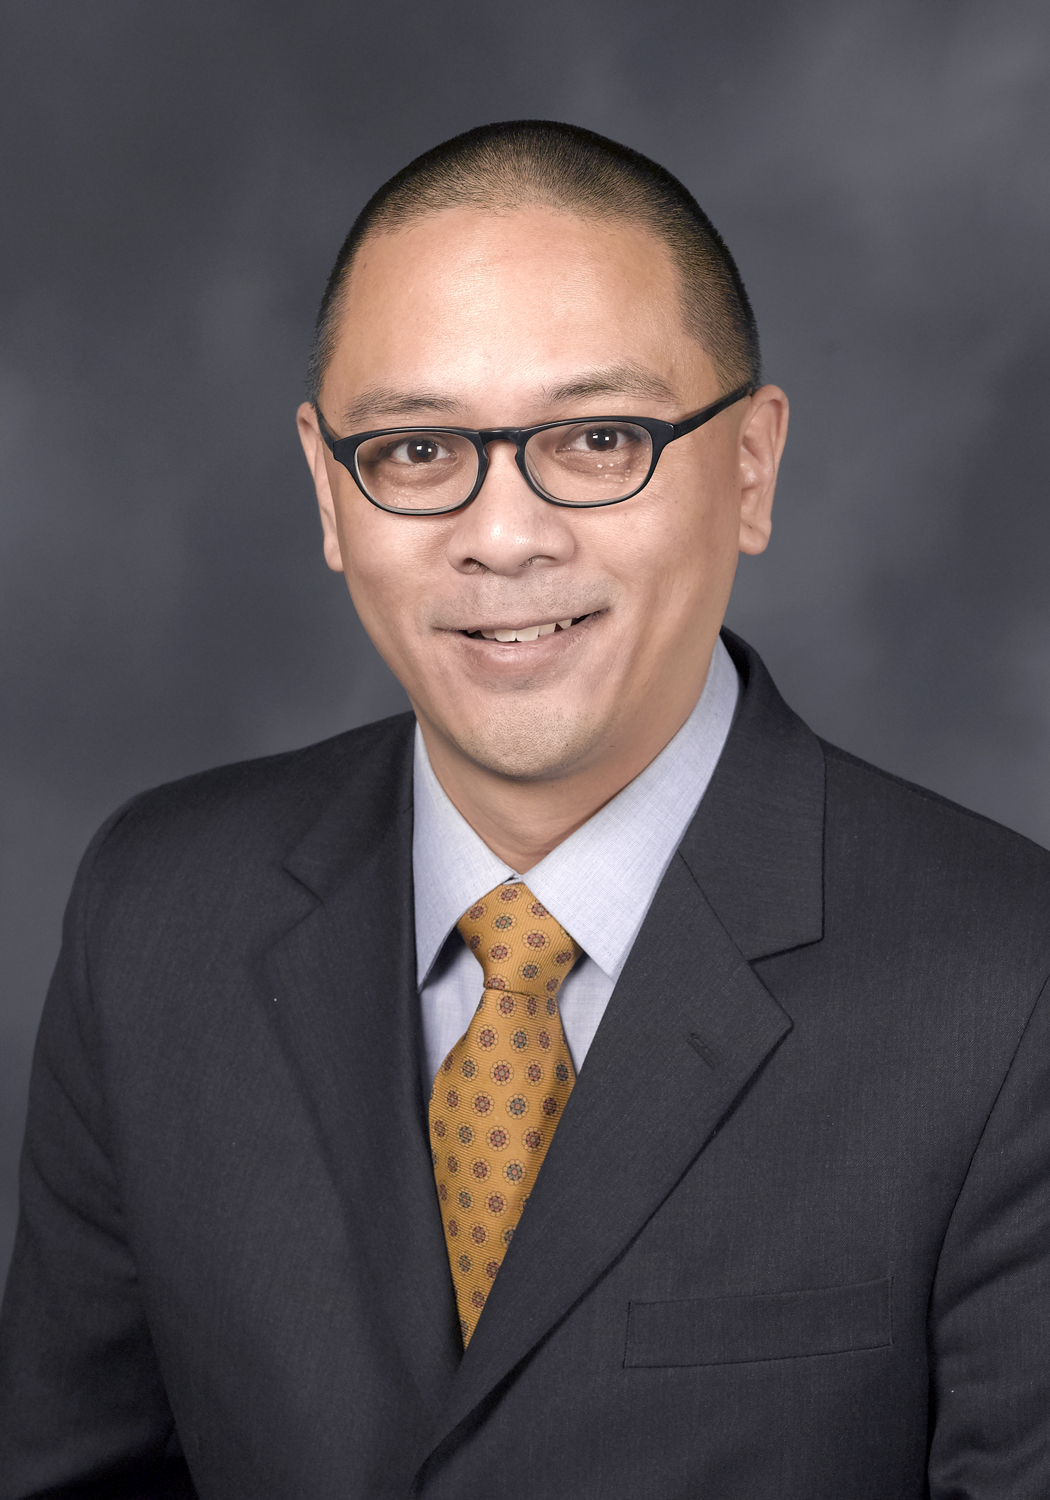
\includegraphics[width=1in,height=1.25in,clip,keepaspectratio]{\myroot/figures/evangelista_d_prof.jpg}}]{Dennis Evangelista} raises guide dog puppies. 
%\end{IEEEbiography}

\end{document}